\renewcommand{\thechapter}{\Alph{chapter}}
\renewcommand{\thefigure}{\Alph{chapter}.\arabic{figure}}
\renewcommand{\chaptername}{Appendix}
\addcontentsline{toc}{part}{Appendix}

\setlength{\beforechapskip}{-60pt}
\setlength{\afterchapskip}{0pt}
\setlength{\footskip}{5cm}

\clearpage
\checkandfixthelayout

\chapter{}\label{apdx:flowchart_a1}
\begin{minipage}{\textwidth}
  \centering
\end{minipage}

\clearpage

\chapter{Vacuum chamber risk assessment}\label{apdx:risk_assessment}
\begin{longtable}{|p{4cm}|p{10cm}|}
\hline
\multicolumn{2}{|c|}{\textbf{Experimental Design for Testing a Barometer in a Vacuum Chamber}} \\
\hline
\textbf{Objective} & Test the accuracy of the barometer in a vacuum chamber using Blue Raven for comparison. Expected pressure readings at 7000 feet will be determined. \\
\hline
\textbf{Expected Pressure Readings} & Approx. 78.36 kPa at an apogee of 7000 feet (2133.6 meters). \\
\hline
\textbf{Equipment Required} & 
\begin{itemize}
    \item Vacuum Chamber (VEVOR 2 Gallon Vacuum Chamber)
    \item Vacuum Pump
    \item Avionics board
    \item Blue Raven Flight computer
    \item Power Supply for electronics
    \item Pfeiffer Vacuum Gauge - \href{https://www.pfeiffer-vacuum.com/en/products/measurement-analysis-and-control/pressure-sensors/ptr-2695-0/ptr26950a/}{PTR26950A} (Borrowed from Glenn Matthews)
\end{itemize} \\
\hline
\textbf{Methodology} & 
\begin{enumerate}
    \item \textbf{Setup}:
    \begin{enumerate}
        \item Connect Pfeiffer gauge to pump and vacuum chamber.
        \item Place the barometer and Blue Raven inside the vacuum chamber.
    \end{enumerate}
    \item \textbf{Initialisation}: Calibrate electronics. Set Blue Raven to ground test mode.
    \begin{itemize}
        \item Start data collection on Avionics board
        \item Trigger launch event on Blue Raven
    \end{itemize}
    \item \textbf{Running the Test}: Gradually reduce pressure, especially near 78.36 kPa.
    \item \textbf{Apogee Simulation}: Decrease pressure to 78.36 kPa and maintain for a couple of seconds.
    \begin{itemize}
        \item This is maintained by decreasing the pressure equal to the amount of pressure leak.
    \end{itemize}
    \item Gradually depressurise chamber to simulate the return to ground.
    \item \textbf{Data Collection}: Collect data and verify Avionics data.
\end{enumerate} \\
\hline
\textbf{Vacuum Pump Controls} & Power on and off. \\
\hline
\textbf{Using Blue Raven for Ground Truths} & Use Blue Raven’s pressure readings as baseline for comparison. Validate barometer accuracy against Blue Raven readings. \\
\hline
\textbf{Leak Rate} & Monitor vacuum chamber for leaks. Calculate leak rate by measuring pressure change over time. \\
\hline
\textbf{Risk Considerations} & See completed risk assessments. \\
\hline
\end{longtable}
\vfill{}

\clearpage

\chapter{Vacuum chamber test ground state}\label{apdx:vacuum_ground-raven}
\vfill{}
\begin{figure}[h]
  \begin{center}
    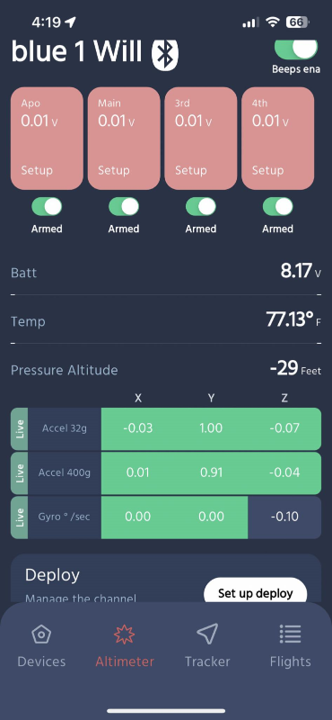
\includegraphics[width=0.55\textwidth]{./img/vacuum_ground-raven.png}
  \end{center}
\end{figure}
\vfill{}

\clearpage

\chapter{Vacuum chamber test apogee}\label{apdx:vacuum_peak-raven}
\vfill{}
\begin{figure}[h]
  \begin{center}
    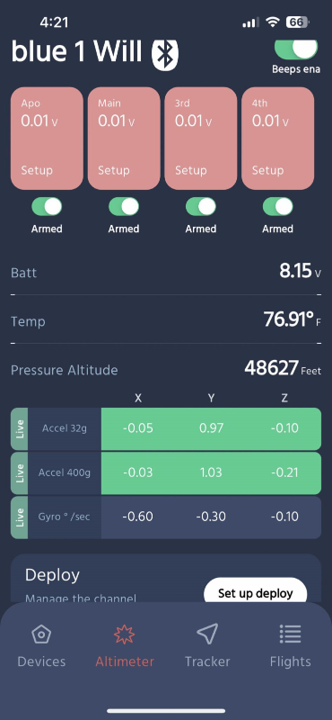
\includegraphics[width=0.55\textwidth]{./img/vacuum_peak-raven.png}
  \end{center}
\end{figure}
\vfill{}

